\documentclass[11pt,a4paper]{article}
\usepackage[margin=25mm]{geometry}
\usepackage{amsmath,amssymb,longtable}
\usepackage{graphicx}
\usepackage{tikz}
\usepackage[hidelinks]{hyperref}
\hypersetup{
  pdftitle={VTOL26: Nine-Actuator Simulation Model},
  pdfauthor={VTOL26},
  pdfsubject={Rigid-body dynamics, actuator forces and configuration parameters}
}
\numberwithin{equation}{section}
\setlength{\emergencystretch}{1em}
\definecolor{forceblue}{RGB}{0,65,130}
\definecolor{anglered}{RGB}{175,35,35}
\definecolor{gravitygreen}{RGB}{25,110,55}

\newcommand{\vect}[1]{\boldsymbol{#1}}
\newcommand{\R}{\mathbb{R}}
\newcommand{\trans}{^{\mathsf T}}

\title{VTOL26: Nine-Actuator Simulation Model}
\author{VTOL26}
\date{20 November 2026}

\begin{document}
\maketitle

\begin{abstract}
This document explains how the nine actuators of VTOL26 produce forces, turn
the aircraft and change its motion. The aircraft has three motors, two front
rotor tilt servos, two ailerons and two V-tail control surfaces. We first
define the directions and variables, then calculate each force, and finally
use Newton's laws to find how the aircraft moves. The same equations describe
simplified hover, transition and forward flight. Aircraft measurements are
still needed to choose the parameters; these equations alone do not prove
that the simulation matches the real aircraft.
\end{abstract}

\section{What the model does}
In control, the \emph{plant} is the system being controlled. Here it is the
aircraft. A controller chooses actuator commands; the plant predicts the
motion those commands produce. This document defines the plant, not the
controller or the objective used by the particle swarm optimizer (PSO).

The model takes three things: the current state $\vect x$, the actuator inputs
$\vect u$, and the aircraft parameters $\Theta$. It returns
$\dot{\vect x}$, the rate at which the state changes:
$(\vect x,\vect u,\Theta)\mapsto\dot{\vect x}$.
For example, velocity is the rate of change of position, and acceleration is
the rate of change of velocity. A simulator uses these rates to advance time.

The calculation follows four steps:
\begin{enumerate}
  \item Use the aircraft's speed and orientation to find the airflow.
  \item Calculate the forces from the motors, wing and control surfaces.
  \item Add the forces and their turning effects, called \emph{moments}.
  \item Use the total force and moment to calculate acceleration and rotation.
\end{enumerate}

We treat the aircraft as one rigid body: its shape, mass and the location of
its center of gravity (CG) within the airframe stay fixed.
Thrust and servo angles change immediately when commanded;
motor and servo delays are not modeled. Inputs are thrusts in newtons and
angles in radians. Converting electrical commands such as PWM or DShot into
these quantities is a separate step.

The force equations come from the earlier analytical model and PSO
code~\cite{analytical,pso,indices}. Each tail servo drives two force terms,
called \emph{cola} (tail) and ruddervator in those sources. A ruddervator is
a V-tail surface that helps control both pitch and yaw. There are only two
tail servos, even though we calculate four tail force terms. Their areas and
coefficients must describe separate parts of the total force, so that the
same physical force is not counted twice. This approximation and its limits
are explained with the tail equations. The motion equations follow the
earlier Simulink model and quaternion reference~\cite{simulink,thesis}.

\clearpage
\section{Where the forces act}
Figure~\ref{fig:dynamics} shows the aircraft and the forces acting on it.
The drawing is adapted from the earlier model~\cite{analytical}.
The next sections define its symbols and positive directions.

\begin{figure}[!ht]
\centering
\resizebox{\linewidth}{!}{%
\begin{tikzpicture}[
  font=\small,
  force/.style={-latex,very thick,forceblue},
  reaction/.style={-latex,thick,forceblue},
  angle/.style={-latex,thick,anglered},
  reference/.style={dashed,thin,black!45},
  axis/.style={-latex,thick,black},
  every node/.style={inner sep=2pt}
]
  \node[inner sep=0] at (0,0)
    {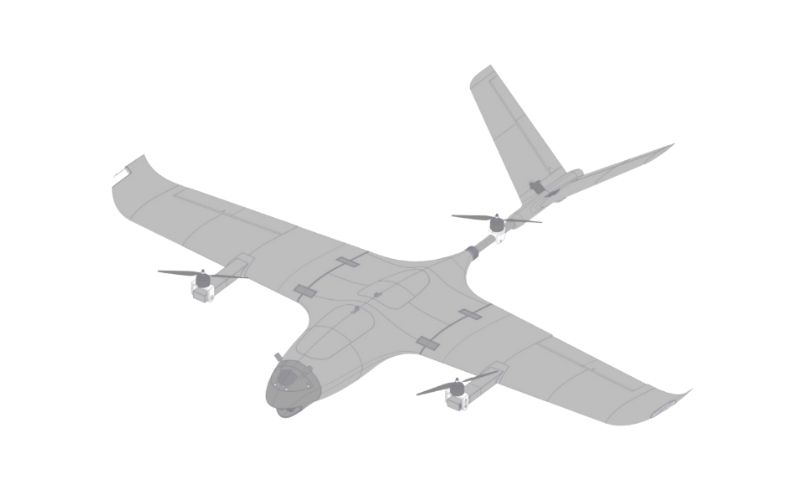
\includegraphics[width=15cm]{vtol_airframe.png}};
  \coordinate (CG) at (-0.1,-0.7);
  \coordinate (ML) at (-3.65,-0.56);
  \coordinate (MR) at (1.13,-2.72);
  \coordinate (MT) at (1.78,0.53);
  \coordinate (AL) at (-4.95,0.34);
  \coordinate (AR) at (3.28,-1.59);
  \coordinate (W) at (-2.44,-0.09);
  \coordinate (HL) at (1.88,2.44);
  \coordinate (HR) at (3.94,1.41);

  % Projected body axes and moments use the document's down-positive convention.
  \draw[reference] (-3.1,-3.0) -- (3.3,2.0);
  \draw[reference] (-5.2,1.15) -- (5.8,-3.25);
  \draw[reference] (-0.1,2.5) -- (-0.1,-3.2);
  \draw[<->,thick] (-3.15,-2.9)
    arc[start angle=180,end angle=505,x radius=0.20,y radius=0.33];
  \node[anchor=east] at (-3.35,-3.05) {$M_{B,x}$};
  \draw[<->,thick] (5.8,-3.12)
    arc[start angle=0,end angle=325,x radius=0.20,y radius=0.33];
  \node[anchor=west] at (6.05,-3.05) {$M_{B,y}$};
  \draw[<->,thick] (-0.1,2.5)
    arc[start angle=90,end angle=415,x radius=0.38,y radius=0.17];
  \node[anchor=south] at (-0.1,2.85) {$M_{B,z}$};

  \draw[axis] (-6.1,-2.7) -- ++(-0.85,-0.65)
    node[anchor=north east] {$x_B$};
  \draw[axis] (-6.1,-2.7) -- ++(1.05,-0.4)
    node[anchor=west] {$y_B$};
  \draw[axis] (-6.1,-2.7) -- ++(0,-1.15)
    node[anchor=north] {$z_B$};
  \node[anchor=south] at (-6.1,-2.5) {body FRD};
  \fill (CG) circle[radius=1.4pt];
  \node[anchor=south west] at (0.02,-0.65) {CG};
  \draw[-latex,very thick,gravitygreen] (CG) -- ++(0,-1.28)
    node[anchor=north east] {$mg$};

  \draw[force] (ML) -- ++(0,1.30) node[anchor=south] {$T_L$};
  \draw[force] (MR) -- ++(0,1.30) node[anchor=south] {$T_R$};
  \draw[force] (MT) -- ++(0,1.18) node[anchor=south west] {$T_T$};
  \draw[reaction] (-3.23,-0.8)
    arc[start angle=0,end angle=-280,x radius=0.37,y radius=0.15];
  \node[forceblue] at (-3.55,-1.26) {$\tau_L$};
  \draw[reaction] (1.55,-2.96)
    arc[start angle=0,end angle=280,x radius=0.37,y radius=0.15];
  \node[forceblue] at (1.33,-3.39) {$\tau_R$};
  \draw[reaction] (2.20,0.25)
    arc[start angle=0,end angle=-280,x radius=0.37,y radius=0.15];
  \node[forceblue] at (2.05,-0.20) {$\tau_T$};

  \draw[force] (W) -- ++(0,1.10) node[anchor=south] {$L_W$};
  \draw[force] (W) -- ++(0.90,0.57) node[anchor=west] {$D_W$};
  \draw[force] (AL) -- ++(0,1.05) node[anchor=south] {$L_{A,L}$};
  \draw[force] (AL) -- ++(0.78,0.49);
  \node[forceblue,anchor=east] at (-5.08,0.83) {$D_{A,L}$};
  \draw[force] (AR) -- ++(0,1.05) node[anchor=south] {$L_{A,R}$};
  \draw[force] (AR) -- ++(0.83,0.52) node[anchor=south west] {$D_{A,R}$};
  \draw[force] (HL) -- ++(0.40,1.03)
    node[anchor=south east] {$L_{C,L}+L_{H,L}$};
  \draw[force] (HL) -- ++(0.90,0.57)
    node[anchor=west] {$D_{C,L}+D_{H,L}$};
  \draw[force] (HR) -- ++(-0.36,1.03)
    node[anchor=south west] {$L_{C,R}+L_{H,R}$};
  \draw[force] (HR) -- ++(0.90,0.57)
    node[anchor=west] {$D_{C,R}+D_{H,R}$};

  \draw[reference,anglered] (ML) -- ++(-0.65,0.65);
  \draw[angle] (-3.65,-0.01)
    arc[start angle=90,end angle=135,radius=0.55];
  \node[anglered,anchor=east] at (-4.18,-0.20) {$\epsilon_L$};
  \draw[reference,anglered] (MR) -- ++(-0.65,0.65);
  \draw[angle] (1.13,-2.17)
    arc[start angle=90,end angle=135,radius=0.55];
  \node[anglered,anchor=east] at (0.62,-2.38) {$\epsilon_R$};

  \draw[reference,anglered] (HL) -- ++(0,0.80);
  \draw[angle] (1.88,3.12)
    arc[start angle=90,end angle=64,radius=0.68];
  \node[anglered,anchor=east] at (1.60,3.02) {$\gamma_L$};
  \draw[reference,anglered] (HR) -- ++(0,0.80);
  \draw[angle] (3.94,2.09)
    arc[start angle=90,end angle=110,radius=0.68];
  \node[anglered,anchor=west] at (4.16,2.28) {$\gamma_R$};

  \draw[angle] (-5.15,0.06)
    arc[start angle=195,end angle=245,x radius=0.45,y radius=0.22];
  \node[anglered,anchor=east] at (-5.28,-0.10) {$\beta_L$};
  \draw[angle] (3.94,-2.04)
    arc[start angle=195,end angle=245,x radius=0.45,y radius=0.22];
  \node[anglered,anchor=west] at (4.15,-2.25) {$\beta_R$};

  \draw[angle,dashed] (CG) -- ++(-1.38,-0.50)
    node[anchor=east] {$\vect v_B$};
  \draw[angle] (-0.78,-1.23)
    arc[start angle=218,end angle=200,radius=0.86];
  \node[anglered] at (-1.07,-1.38) {$\alpha$};
\end{tikzpicture}%
}
\caption{Forces and angles on the aircraft. Blue arrows show forces and motor
reaction torques; red marks show angles; green shows weight. Black and gray
marks show body axes and moments. The rotors are drawn with zero tilt.
The aerodynamic arrows show example directions; a negative calculated value
reverses the corresponding lift direction.}
\label{fig:dynamics}
\end{figure}
Count three thrusts, two rotor tilt angles and four control-surface angles:
these are the nine inputs. Each tail label combines the two force terms
driven by the same servo angle $\gamma_i$. The curved motor arrows show the
reaction torque $\tau_i=\kappa_iT_i$, caused by spinning the propellers.
The drawing only shows the arrangement. Use the configured distances from
the CG when calculating moments; do not measure distances from this image.
\clearpage

\section{Directions, signs and variables}
\subsection{Two coordinate systems}
We need one set of axes attached to the ground and another attached to the
aircraft. These coordinate systems are called \emph{reference frames}.
We use the same directions as PX4:
\begin{itemize}
  \item $N$: north--east--down (NED). Its origin stays fixed on the ground.
  We treat it as an inertial frame, so we can apply Newton's laws in it.
  Position and velocity use these axes. A larger down coordinate means a
  lower altitude.
  \item $B$: forward--right--down (FRD). Its origin is the aircraft's CG,
  and its axes turn with the aircraft. Forces and moments use these axes.
  Here $x_B$ points toward the nose, $y_B$ toward the right wing, and $z_B$
  toward the underside. A point on the left has $y_B<0$.
\end{itemize}
``Down'' in the body frame means toward the aircraft's underside, even when
the aircraft is tilted. Gravity always points down in the ground frame:
\begin{equation}
  \vect g_N=\begin{bmatrix}0&0&g\end{bmatrix}\trans,\qquad g>0.
\end{equation}
Here $g$ is gravitational acceleration in m/s$^2$.
Both frames follow the right-hand rule: point your right thumb along a
positive axis, and your curled fingers show positive rotation about it.
Positive roll about $x_B$ lowers the right wing; positive pitch about $y_B$
raises the nose; positive yaw about $z_B$ turns the nose right.

Bold symbols are vectors. Their entries are written as columns; the
superscript $\mathsf T$ means transpose, which turns a row into a column or
reverses that operation. A subscript $N$ or $B$ says which axes a vector uses.
The side labels $L,R,T$ mean left, right and rear rotor.
The labels $W,A,C,H$ mean wing, aileron, \emph{cola} and ruddervator.

\subsection{State}
The \emph{state} collects what we need to know about the aircraft right now:
where it is, how fast it moves, which way it points and how fast it rotates.
\begin{equation}\label{eq:state}
  \vect x=
  \begin{bmatrix}\vect p_N\trans&\vect v_N\trans&q\trans&\vect\omega_B\trans\end{bmatrix}\trans
  \in\R^{13},\qquad
  q=\begin{bmatrix}q_0&q_1&q_2&q_3\end{bmatrix}\trans,\quad q\trans q=1.
\end{equation}
\begin{center}
\begin{tabular}{lll}
\hline
Variable & Meaning & Units \\
\hline
$\vect p_N=(p_N,p_E,p_D)\trans$ & CG position in NED & m \\
$\vect v_N$ & CG velocity in NED & m/s \\
$q$ & Orientation, stored as a quaternion & dimensionless \\
$\vect\omega_B=(\omega_x,\omega_y,\omega_z)\trans$ & Roll, pitch and yaw rates about body axes & rad/s \\
\hline
\end{tabular}
\end{center}
There are thirteen stored numbers: three for position, three for velocity,
four for orientation and three for angular velocity.
A \emph{quaternion} stores orientation without the ambiguity that roll and
yaw angles have when pitch reaches $90^\circ$. Its four numbers must
satisfy $q\trans q=1$, meaning their squares add to one. We use the Hamilton
convention with the scalar $q_0$ first; $q$ rotates body vectors into NED.
The next section gives the formulas needed to use it.

The components of $\vect\omega_B$ are rotation rates about the aircraft's
current axes. They are not generally the time derivatives of Euler angles.
They are also unrelated to the motor commands named \texttt{omega} in PSO.

\subsection{Nine physical actuator inputs}
The \emph{input} is what we command. The order below matches PSO, with its
first three commands converted into thrust:
\begin{equation}\label{eq:inputs}
  \vect u=
  \begin{bmatrix}
    T_L&T_R&T_T&\epsilon_L&\epsilon_R&\gamma_L&\gamma_R&\beta_L&\beta_R
  \end{bmatrix}\trans\in\R^9.
\end{equation}
\begin{center}
\begin{tabular}{clll}
\hline
PSO index & Input & Actuator & Units \\
\hline
0 & $T_L$ & Left-front motor thrust & N \\
1 & $T_R$ & Right-front motor thrust & N \\
2 & $T_T$ & Rear motor thrust & N \\
3 & $\epsilon_L$ & Left-front rotor tilt servo & rad \\
4 & $\epsilon_R$ & Right-front rotor tilt servo & rad \\
5 & $\gamma_L$ & Left ruddervator servo & rad \\
6 & $\gamma_R$ & Right ruddervator servo & rad \\
7 & $\beta_L$ & Left aileron servo & rad \\
8 & $\beta_R$ & Right aileron servo & rad \\
\hline
\end{tabular}
\end{center}
The plant expects the first three inputs in newtons. If using PSO motor
commands $w_i$, convert them first with the existing linear rule:
\begin{equation}\label{eq:pso-map}
  T_i=k_T w_i,\qquad i\in\{L,R,T\},
\end{equation}
The factor $k_T$ gives newtons per command unit and is shared by the three
motors in the existing code~\cite{pso,config}. The units of $w_i$ still need
to be established: the name \texttt{omega} alone does not mean rad/s, RPM
or microseconds. This conversion preserves the current approximation;
this document supplies no motor measurements to validate it.

Thrust cannot be negative. At zero tilt, a rotor pushes upward along $-z_B$.
At $\epsilon_i=\pi/2$ ($90^\circ$), a front rotor pushes forward along $+x_B$.
The force equations below define positive tail and aileron angles. In
particular, PSO uses opposite lift signs for the left and right ailerons.
Servo reversal and neutral offsets must be handled when converting an
electrical command into the physical angle.

Each input has a minimum and maximum:
$\vect u_{\min}\leq\vect u\leq\vect u_{\max}$, applied entry by entry.
Before calculating forces, the simulator must either reject inputs outside
these limits or clip them to the nearest allowed value. Use one policy
consistently.

\section{Converting between ground and body axes}
A force pointing up from the aircraft may point partly sideways relative
to the ground when the aircraft banks. A \emph{rotation matrix} converts
the components between the two sets of axes without changing the vector
itself. Here $R(q)$ converts body components into NED, and its transpose
$R(q)\trans$ converts NED components back into body components.

The following formulas define our quaternion convention. You can follow
the force model using $R(q)$ without working through the quaternion algebra.
For two quaternions $a=(a_0,\vect a)$ and $b=(b_0,\vect b)$, the symbol
$\otimes$ means quaternion multiplication:
\begin{equation}
 a\otimes b=
 \begin{bmatrix}
 a_0b_0-\vect a\trans\vect b\\
 a_0\vect b+b_0\vect a+\vect a\times\vect b
 \end{bmatrix},\qquad q^*=(q_0,-q_1,-q_2,-q_3)\trans.
\end{equation}
Here $q^*$ is the \emph{conjugate}: keep the first entry and reverse the
other three signs. The dot product $\vect a\trans\vect b$ gives a scalar;
the cross product $\vect a\times\vect b$ gives a vector perpendicular to both.
Writing a three-component vector as $[0,\vect z_B]$ lets us rotate it with
quaternions: $[0,\vect z_N]=q\otimes[0,\vect z_B]\otimes q^*$.
The same operation, written as a matrix, is
\begin{equation}\label{eq:rotation}
R(q)=\begin{bmatrix}
1-2(q_2^2+q_3^2)&2(q_1q_2-q_0q_3)&2(q_1q_3+q_0q_2)\\
2(q_1q_2+q_0q_3)&1-2(q_1^2+q_3^2)&2(q_2q_3-q_0q_1)\\
2(q_1q_3-q_0q_2)&2(q_2q_3+q_0q_1)&1-2(q_1^2+q_2^2)
\end{bmatrix}.
\end{equation}
Thus $\vect z_N=R(q)\vect z_B$ and
$\vect z_B=R(q)\trans\vect z_N$ for any vector $\vect z$.
For example, $q=(1,0,0,0)\trans$ makes $R(q)$ the identity matrix:
the nose points north, the right wing points east, and both down axes agree.

We also need matrices that rotate a vector through an angle $\theta$ about
the $x$ or $y$ axis. Positive angles follow the same right-hand rule:
\begin{equation}\label{eq:elementary}
 R_x(\theta)=\begin{bmatrix}
 1&0&0\\0&\cos\theta&-\sin\theta\\0&\sin\theta&\cos\theta
 \end{bmatrix},\qquad
 R_y(\theta)=\begin{bmatrix}
 \cos\theta&0&\sin\theta\\0&1&0\\-\sin\theta&0&\cos\theta
 \end{bmatrix}.
\end{equation}
Use these conventions for every state input. NED position, FRD angular
velocity and a body-to-NED quaternion can be used directly. Changing only
the sign of position Z is not enough to convert a state from another
coordinate convention; velocity, orientation and angular velocity must agree.

\section{Speed, angle of attack and aerodynamic coefficients}
The model assumes still air. The aircraft's velocity relative to the air
therefore equals its velocity relative to the ground. Express that velocity
in body axes to find its speed $V$ and angle of attack $\alpha$:
\begin{align}
 \vect v_B&=R(q)\trans\vect v_N=(v_x,v_y,v_z)\trans,\\
 V&=\|\vect v_B\|,\qquad Q=\tfrac12\rho V^2,\label{eq:pressure}\\
 \alpha&=\begin{cases}
   \operatorname{atan2}(v_z,v_x),&(v_x,v_z)\ne(0,0),\\
   0,&(v_x,v_z)=(0,0).
 \end{cases}\label{eq:alpha}
\end{align}
The notation $\|\vect v_B\|$ means the vector's length, so $V$ is speed
in m/s. Air density is $\rho>0$. The quantity $Q$, called \emph{dynamic
pressure}, measures the strength of the airflow and is in pascals (Pa).
It grows with speed squared: doubling speed gives four times $Q$.
All aerodynamic forces below contain this factor.

Angle of attack $\alpha$ is the angle, in radians, between the forward
body axis and the velocity in the body's $x$--$z$ plane.
The function $\operatorname{atan2}$ finds the angle while keeping track of
the quadrant. For forward motion, $v_z>0$ gives positive $\alpha$:
the nose points above the direction of travel. When both $v_x$ and $v_z$
are zero, we set $\alpha=0$. At zero speed, $Q=0$, so every aerodynamic
force is zero regardless of this angle choice.

All surfaces use this same airflow estimate. The model does not separately
calculate forces from sideways airflow (sideslip), the different local
velocities caused by aircraft rotation, or air blown over surfaces by the
propellers (propwash).

An aerodynamic coefficient describes how much lift or drag an area produces
at a given $Q$. For the wing, the existing models~\cite{pso,symbolic} use
\begin{equation}\label{eq:wing-coeff}
 C_{L,W}=C_{L0,W}+C_{L\alpha,W}\alpha,\qquad
 C_{D,W}=C_{D0,W}+K_W C_{L,W}^2.
\end{equation}
The first equation says that the lift coefficient $C_{L,W}$ starts at
$C_{L0,W}$ when $\alpha=0$ and changes linearly with $\alpha$.
The slope $C_{L\alpha,W}$ tells us how quickly it changes.
The second equation starts drag at $C_{D0,W}$ and adds drag as lift grows;
$K_W$ sets the size of that extra term.

The control surfaces below also use constant lift and drag slopes, as in PSO.
These constants need to be chosen from measurements or other aerodynamic
data. The earlier analytical source allows more detailed coefficient curves
but does not provide measured ones, so none are added here.

\section{Calculating the forces}
We now calculate the force of each motor and aerodynamic surface.
Every force is a three-component vector in body axes, in newtons.
Gravity will be added later, in the motion equations.

\subsection{Three motors and two tilt servos}
For a motor, force is thrust magnitude $T_i$ times a unit direction vector
$\vect a_i$. The front tilt angle changes that direction:
\begin{align}
 \vect a_i&=R_y(-\epsilon_i)\begin{bmatrix}0\\0\\-1\end{bmatrix}
 =\begin{bmatrix}\sin\epsilon_i\\0\\-\cos\epsilon_i\end{bmatrix},
 &\vect F_{M,i}&=T_i\vect a_i,\quad i\in\{L,R\},\label{eq:front}\\
 \vect a_T&=\begin{bmatrix}0\\0\\-1\end{bmatrix},
 &\vect F_{M,T}&=T_T\vect a_T.\label{eq:rear}
\end{align}
Each $\vect a_i$ has length one. At zero tilt, the front force is
$(0,0,-T_i)\trans$: all thrust points upward. At $90^\circ$, it is
$(T_i,0,0)\trans$: all thrust points forward. Between these angles,
thrust has both upward and forward components. Changing direction also
changes the motor's turning effect about the CG. The rear rotor always
pushes upward and has no tilt servo.

\subsection{Wing}
Lift acts perpendicular to the direction of travel in the $x$--$z$ plane;
drag opposes travel in that plane. Their values come from dynamic pressure
times wing area $S_W$ times the corresponding coefficient.
We then rotate the lift and drag into body axes:
\begin{equation}\label{eq:wing}
 L_W=QS_W C_{L,W},\qquad D_W=QS_W C_{D,W},\qquad
 \vect F_W=R_y(-\alpha)\begin{bmatrix}-D_W\\0\\-L_W\end{bmatrix}.
\end{equation}
Multiplying out the rotation gives
\begin{equation}
 \vect F_W=\begin{bmatrix}
  -D_W\cos\alpha+L_W\sin\alpha\\
  0\\
  -D_W\sin\alpha-L_W\cos\alpha
 \end{bmatrix}.
\end{equation}
At $\alpha=0$, this becomes $(-D_W,0,-L_W)\trans$: drag points backward
and positive lift points upward. At other angles, each has both X and Z
components. A negative $L_W$ means lift acts in the opposite direction.
When implementing this, a force vector has three entries $[F_x,F_y,F_z]$;
the quaternion form $[0,F_x,F_y,F_z]$ has an extra leading zero.

\subsection{Two independent ailerons}
Ailerons change the lift on the two sides of the wing and can make the
aircraft roll. We calculate the \emph{extra} lift and drag caused by moving
each aileron away from neutral. Here $S_A$ is the area of one aileron.
The factor $\eta_L=-1$, $\eta_R=+1$ keeps PSO's left/right command signs:
\begin{align}
 L_{A,i}&=\eta_i QS_A C_{L\beta,A}\beta_i,&
 D_{A,i}&=QS_A C_{D\beta,A}|\beta_i|,\label{eq:aileron-mag}\\
 \vect F_{A,i}&=R_y(-\alpha)
 \begin{bmatrix}-D_{A,i}\\0\\-L_{A,i}\end{bmatrix},&& i\in\{L,R\}.
 \label{eq:aileron-force}
\end{align}
The constants $C_{L\beta,A}$ and $C_{D\beta,A}$ set the extra lift and drag
per radian of deflection. Lift can be positive or negative. Drag uses
$|\beta_i|$, the absolute angle, so moving either way adds drag when the
drag slope is nonnegative.

The two commands are independent. Equal positive commands produce opposite
lift changes because of $\eta_i$; the command signs do not mean identical
physical hinge directions on both sides. At neutral, these extra forces are
zero. The baseline wing force already includes the neutral aileron area,
so that area must not be counted again.

\subsection{Two tail servos}
The two V-tail panels produce both upward and sideways force because they
are tilted. This lets the tail affect both pitch and yaw.
For each side, we keep the earlier model's two force terms: $C$ for
\emph{cola} and $H$ for ruddervator. Both use the same servo command:
\begin{equation}\label{eq:tail-coupling}
 \delta_{C,L}=\delta_{H,L}=\gamma_L,\qquad
 \delta_{C,R}=\delta_{H,R}=\gamma_R.
\end{equation}
The symbols $\delta_{C,i}$ and $\delta_{H,i}$ are just names for that shared
angle, not extra commands. In the original analytical model, the ruddervator
uses a local airflow angle plus its deflection,
$\alpha_{\mathrm{rud},i}+\gamma_{\mathrm{rud},i}$.
PSO replaces that whole angle with $\gamma_i$~\cite{pso}, and we keep that
simplification here. There is no separately calculated local tail angle.

Use $X\in\{C,H\}$ to mean ``apply this equation once to each tail force
term.'' For each term, $S_X$ is the area on one side, and $\chi_X$ is its
upward tilt angle, or \emph{cant}, measured from horizontal.
The matrices $H_{X,i}$ tilt the force in opposite directions on the two sides:
\begin{equation}\label{eq:tail-rotation}
 H_{X,L}=R_x(+\chi_X),\qquad H_{X,R}=R_x(-\chi_X).
\end{equation}
The panels extend outward and upward from the centerline. Positive lift on
the left panel points up and right; positive lift on the right points up
and left. Calculate lift and drag, then use $H_{X,i}$ to put them in body axes:
\begin{align}
 L_{X,i}&=QS_X C_{L\gamma,X}\gamma_i,&
 D_{X,i}&=QS_X C_{D\gamma,X}|\gamma_i|,\label{eq:tail-mag}\\
 \vect F_{X,i}&=H_{X,i}
 \begin{bmatrix}-D_{X,i}\\0\\-L_{X,i}\end{bmatrix},&&
 X\in\{C,H\},\quad i\in\{L,R\}.\label{eq:tail-force}
\end{align}
The constants $C_{L\gamma,X}$ and $C_{D\gamma,X}$ give the lift and drag
per radian of command. As with the ailerons, the absolute angle in the drag
term makes either direction of deflection add drag.
Writing out the body components shows the sideways-force signs:
\begin{equation}
 \vect F_{X,L}=\begin{bmatrix}
 -D_{X,L}\\ L_{X,L}\sin\chi_X\\-L_{X,L}\cos\chi_X
 \end{bmatrix},\qquad
 \vect F_{X,R}=\begin{bmatrix}
 -D_{X,R}\\-L_{X,R}\sin\chi_X\\-L_{X,R}\cos\chi_X
 \end{bmatrix}.
\end{equation}
The $C$ and $H$ terms may have different areas, slopes, cant angles and
force locations. They still respond to only two servos. Each equation is
already for one side; do not multiply it by two.

This approximation has an important limit: when both tail commands are
zero, all four tail forces are zero, even if the aircraft has a nonzero
angle of attack. A real fixed tail can produce force in that condition.
This behavior comes from PSO's shared-command approximation. The tail
forces here also use body X for drag and the fixed cant rotation for lift;
they do not use the wing's $R_y(-\alpha)$ rotation.

\section{Adding forces and turning effects}
\subsection{Total force}
All forces now use body axes, so we can add their X, Y and Z components.
The symbol $\sum$ means ``add over the listed components'':
\begin{equation}\label{eq:force-sum}
 \vect F_B=\vect F_W+
 \sum_{i\in\{L,R,T\}}\vect F_{M,i}+
 \sum_{i\in\{L,R\}}
 \left(\vect F_{A,i}+\vect F_{C,i}+\vect F_{H,i}\right).
\end{equation}
There are ten force terms: one wing, three motors, two ailerons and four
tail terms. There are still nine actuator inputs, because one input can
affect more than one force. Gravity is not included in $\vect F_B$.

\subsection{Total moment about the CG}
A force can also turn the aircraft if it acts away from the CG, just as a
push turns a door more easily when applied far from the hinge.
For force $\vect F_k$, the vector
$\vect r_k=(r_{k,x},r_{k,y},r_{k,z})\trans$ points from the CG to where
that force acts. Both vectors use body axes. The moment is their cross
product $\vect r_k\times\vect F_k$, measured in newton-metres (N m).
The index $k$ runs over these ten components:
\begin{equation}
 \mathcal K=\{W,M_L,M_R,M_T,A_L,A_R,C_L,C_R,H_L,H_R\}.
\end{equation}
Motors add another turning effect: the aircraft feels a reaction torque
as each motor drives its propeller. Following the analytical
model~\cite{analytical}, we approximate its size as proportional to thrust.
Add these reaction torques along the rotor axes to the moments from forces:
\begin{equation}\label{eq:moment-sum}
 \vect M_B=\sum_{k\in\mathcal K}\vect r_k\times\vect F_k+
 \sum_{i\in\{L,R,T\}}\kappa_i T_i\vect a_i.
\end{equation}
The first sum is the moment from forces acting away from the CG. The second
is motor reaction torque. The factor $\kappa_i$ is reaction torque divided
by thrust, so its unit is metres. Its sign must match the motor and
propeller spin direction. When a front rotor tilts, its reaction torque
tilts with it. With vertical rotors, this torque acts about the yaw axis.
Setting every $\kappa_i=0$ omits this effect, as the current PSO does.

The cross product can also be written one component at a time:
\begin{align}
 M_{B,x}^{\mathrm{arm}}&=\sum_k(r_{k,y}F_{k,z}-r_{k,z}F_{k,y}),\\
 M_{B,y}^{\mathrm{arm}}&=\sum_k(r_{k,z}F_{k,x}-r_{k,x}F_{k,z}),\\
 M_{B,z}^{\mathrm{arm}}&=\sum_k(r_{k,x}F_{k,y}-r_{k,y}F_{k,x}).
\end{align}
For example, an upward force $T$ at $(r_x,r_y,0)\trans$ gives a moment
$(-r_yT,r_xT,0)\trans$. On the right side, $r_y>0$, so upward thrust
produces negative roll moment: it raises the right wing.
If the force acts at the CG, $\vect r_k=0$, so its lever-arm moment is zero.
Motor reaction torque can still remain.

Add the motor reaction components to these three equations once.
The force moments already include the roll, pitch and yaw effects drawn
separately in the original source; adding those again would double-count
them. This model has no other direct moment term.

\section{From forces to motion}
We now have total force $\vect F_B$ and total moment $\vect M_B$.
Newton's laws turn them into changes in the state. A dot means a time
derivative. The mass $m$ and inertia matrix $J$ are constant:
\begin{align}
 \dot{\vect p}_N&=\vect v_N,\label{eq:position-dot}\\
 \dot{\vect v}_N&=\frac{1}{m}R(q)\vect F_B+\vect g_N,\label{eq:velocity-dot}\\
 \dot q&=\tfrac12 q\otimes\begin{bmatrix}0\\\vect\omega_B\end{bmatrix},
 \label{eq:quaternion-dot}\\
 \dot{\vect\omega}_B&=J^{-1}
 \left(\vect M_B-\vect\omega_B\times(J\vect\omega_B)\right).
 \label{eq:angular-dot}
\end{align}
Read the four equations as follows:
\begin{enumerate}
  \item \textbf{Position changes with velocity.} This is the definition of
  velocity, applied to the three NED position components.
  \item \textbf{Velocity changes with acceleration.} Rotate the force into
  NED, divide by mass, and add gravitational acceleration. This is
  $\text{acceleration}=\text{force}/\text{mass}$ in ground axes.
  \item \textbf{Orientation changes with angular velocity.} The quaternion
  equation updates which way the aircraft points using its current body
  rotation rates.
  \item \textbf{Angular velocity changes with moment.} Inertia describes
  resistance to angular acceleration, much as mass describes resistance to
  linear acceleration. The term
  $\vect\omega_B\times(J\vect\omega_B)$ accounts for the coupling between
  rotation about different axes. At zero angular velocity it is zero.
\end{enumerate}

We use $J=\operatorname{diag}(J_x,J_y,J_z)$: a matrix with the three
inertias on the diagonal and zeros elsewhere, as in the earlier model.
The mass, CG and
inertias must all describe the same assembled aircraft.
The aircraft has six degrees of freedom: three for position and three for
orientation. Storing orientation as four quaternion entries does not add
another physical freedom; their unit-length constraint must be maintained.

Gravity enters only through Equation~\eqref{eq:velocity-dot}. Weight acts
at the CG, so it adds no moment about the CG.
If Gazebo or another physics engine already updates the rigid body and
applies gravity, give it only the force and moment. In a world frame aligned
with NED, these are $R(q)\vect F_B$ and $R(q)\vect M_B$.
Together they are called a \emph{wrench}. Do not add gravity to that force
or run a second motion integrator. If the engine uses other world axes,
convert both vectors to those axes first.

\section{Parameters you must supply}
The equations describe the structure of the model. The parameters below
make it describe a particular aircraft. Together they form $\Theta$.
Measure them, estimate them from CAD or aerodynamic data, or choose them
explicitly for a simulation experiment. Existing configuration-file values
should not be treated as measured calibration without supporting evidence.
Use the same values in the simulator and in any optimizer predicting its
behavior.

\small
\begin{longtable}{p{0.24\textwidth}p{0.12\textwidth}p{0.55\textwidth}}
\hline
Quantity & Units & Meaning and how to choose it \\
\hline
\endfirsthead
\hline
Quantity & Units & Meaning and how to choose it \\
\hline
\endhead
$m$ & kg & Mass of the assembled aircraft. Measure it; it must be positive. \\
$J_x,J_y,J_z$ & kg m$^2$ & Resistance to rotation about each body axis at the CG. Obtain from CAD or measurement; all must be positive. \\
$\vect r_k$, $k\in\mathcal K$ & m & Locations of the ten forces, measured from the same CG. Use each surface's aerodynamic center as its fixed force location in this approximation. \\
$\rho$, $g$ & kg/m$^3$, m/s$^2$ & Air density and gravitational acceleration for the chosen environment; both positive. \\
$S_W$ & m$^2$ & Total reference area of the neutral wing. \\
$S_A,S_C,S_H$ & m$^2$ & Area on one side for each surface force term. The two tail terms must not count the same force twice. \\
$\chi_C,\chi_H$ & rad & Upward tilt angles of the tail terms. Use the full geometric angle, not the half angle used inside a quaternion. \\
$C_{L0,W},C_{D0,W},K_W$ & 1 & Wing lift coefficient at zero angle of attack, baseline drag coefficient, and the factor for extra drag as lift grows. Obtain from aerodynamic data. \\
$C_{L\alpha,W}$ & rad$^{-1}$ & Change in wing lift coefficient per radian of angle of attack. \\
$C_{L\beta,A},C_{D\beta,A}$ & rad$^{-1}$ & Aileron lift and drag coefficient slopes per radian. The left/right lift sign is already in $\eta_i$. \\
$C_{L\gamma,C},C_{D\gamma,C}$ & rad$^{-1}$ & Lift and drag coefficient slopes of the cola term per radian of tail command. \\
$C_{L\gamma,H},C_{D\gamma,H}$ & rad$^{-1}$ & Lift and drag coefficient slopes of the ruddervator term per radian of the same command. \\
$\kappa_L,\kappa_R,\kappa_T$ & m & Motor reaction torque divided by thrust. Obtain from propulsion data, with signs matching propeller spin. \\
$\vect u_{\min},\vect u_{\max}$ & N, rad & Limits for all nine inputs, from motor capability and calibrated servo angles, signs and neutral settings. \\
$k_T$ (PSO only) & N/$U_w$ & Converts PSO motor commands to thrust; $U_w$ is the command unit. This is not another plant input or state. \\
\hline
\end{longtable}
\normalsize
All parameters must be finite. Areas, $C_{D0,W}$, $K_W$ and the drag slopes
must be nonnegative so drag cannot become a forward push.
For the V-tail shown here, $0\leq\chi_X<\pi/2$.
Using one set of surface parameters for both sides assumes left/right
aerodynamic symmetry, as in PSO.
The inertias must also be physically possible: each must be no greater than
the sum of the other two, for example $J_x\leq J_y+J_z$.

Separately, choose the initial position, velocity, quaternion and angular
velocity, plus a positive simulation time step $h$.
The initial quaternion must be nonzero; divide it by its length before use.
Input limits must allow the flight condition being tested. If the motors
and servos cannot balance the aircraft within those limits, running more
optimizer iterations will not make that balance possible.

\section{Using the model in a simulation}
\subsection{One calculation of the state rates}
Given the current state $\vect x$, inputs $\vect u$ and parameters $\Theta$:
\begin{enumerate}
 \item Check that the state and parameters are valid. Divide the nonzero
 quaternion by its length before using it for rotations, and enforce the
 input limits. Convert PSO motor commands to thrust first if needed.
 \item Calculate $R(q)$, $\vect v_B$, $V$, $\alpha$ and $Q$ from
 Equations~\eqref{eq:rotation}--\eqref{eq:alpha}.
 \item Calculate the motor, wing, aileron and tail forces from
 Equations~\eqref{eq:front}--\eqref{eq:tail-force}.
 \item Add the forces and moments to obtain $\vect F_B$ and $\vect M_B$ using
 Equations~\eqref{eq:force-sum} and~\eqref{eq:moment-sum}.
 \item Return the thirteen state rates from
 Equations~\eqref{eq:position-dot}--\eqref{eq:angular-dot}.
\end{enumerate}
A numerical integrator uses these rates to advance the state through time.
For example, a simple Euler step adds $h\dot{\vect x}$ to the current state.
If the chosen integrator evaluates intermediate states, repeat the force
calculation at each of those states. After each completed time step,
divide the quaternion by its length again to keep it a valid orientation.
Reject a zero quaternion or one with nonfinite entries; it cannot represent
an orientation.

There are no extra motor or servo states to advance. There is also no
hover/forward-flight mode switch inside the plant: the forces change as
speed, orientation and actuator inputs change.

\subsection{Hover, transition and forward flight}
At zero airspeed, $Q=0$, so the wing and control surfaces produce no force
in this model. The rotors must support the aircraft.
To hover without drifting or rotating, total force including weight must
be zero, and total moment must be zero. Finding inputs and an attitude that
meet these conditions is called finding a \emph{trim}:
\begin{equation}\label{eq:hover-trim}
 \vect v_N=0,\quad\vect\omega_B=0,\quad
 R(q)\vect F_B+m\vect g_N=0,\quad\vect M_B=0.
\end{equation}
For a level aircraft with vertical rotors, thrust must equal weight:
$T_L+T_R+T_T=mg$. But this alone does not ensure hover. Unequal moments
can still make the aircraft rotate, even when total thrust equals weight.
Both the force moments and motor reaction torques must balance. Depending
on geometry and propeller spin directions, hover may require some front
rotor tilt or a different aircraft attitude.

During transition, the front rotors tilt forward and start accelerating the
aircraft. As speed rises, $Q$ rises and the wing can carry more of the
weight. The equations calculate both effects at the same time.
In forward flight, the front rotors can approach $90^\circ$ tilt and rear
thrust can decrease if its limits allow it. Straight flight at constant
velocity still needs total force, including weight, and total moment to
balance.

These equations let us study all three flight conditions, but they do not
prove that a stable transition is possible. The model omits stall,
propwash, aerodynamic delays, aerodynamic damping caused by rotation,
ground contact, wind, and motor or servo response times.
The linear lift equations are useful only over the angle range supported
by their aerodynamic data. In particular, they keep increasing lift where
a real wing may stall. Choosing plausible mass and thrust values does not
make those missing effects appear.

\subsection{Simple checks before testing a controller}
These checks help catch wrong signs, missing terms and integration errors.
Use the same parameter set as the simulation:
\begin{enumerate}
 \item \textbf{Free fall.} Start at rest with zero thrust and zero surface
 angles. Then $\dot{\vect v}_N=\vect g_N$: down velocity must increase.
 \item \textbf{Rotor direction.} At zero tilt, a rotor must give $F_z=-T$.
 At $90^\circ$, a front rotor must give $F_x=T$ and $F_z=0$.
 \item \textbf{Wing direction.} For forward flight with $\alpha=0$, drag
 must point along negative X and positive lift along negative Z.
 With no sideways velocity,
 $\vect F_W\trans\vect v_B=-D_W V$: drag removes kinetic energy, while
 lift is perpendicular to velocity and does no work on the aircraft's
 translational motion.
 \item \textbf{Tail symmetry.} With matching left/right parameters and
 $\gamma_L=\gamma_R$, sideways tail forces must cancel. With equal and
 opposite commands, vertical lift terms must cancel; drag terms still add.
 \item \textbf{Moment signs.} Vertical thrust at $(r_x,r_y,0)$ must give
 lever-arm moment $(-r_yT,r_xT,0)\trans$, plus any motor reaction torque.
 Moving a force to the CG removes its lever-arm moment only.
 \item \textbf{Balance and time step.} Check all trim conditions, including
 moment balance. Keep the quaternion at unit length. Reduce the time step
 and check that the results approach the same motion.
\end{enumerate}
Passing these checks shows that the implementation follows the equations.
It does not show that the parameters or predicted aircraft behavior are
accurate.

\clearpage
\section{Notes for comparing with the earlier models}
This section is useful when reading the older documents or source code.
It can be skipped on a first reading. The equations above bring those sources
together with consistent axes and units; the existing PSO code does not
necessarily implement every equation exactly as written here.

The labels in the original \texttt{VTOL.zip} correspond to these labels:
\begin{center}
\begin{tabular}{ll}
\hline
Original source & Present notation \\
\hline
$f_1,f_2,f_3$ & $T_R,T_L,T_T$ \\
$\epsilon_1,\epsilon_2$ & $\epsilon_R,\epsilon_L$ \\
$L_1,L_4$ and $D_1,D_4$ & Combined wing $L_W,D_W$ \\
$L_2,L_3$ and $D_2,D_3$ & Right/left aileron forces \\
$L_5,L_6$ and $D_5,D_6$ & Right/left combined tail forces \\
$\gamma_1,\gamma_2$ & $\gamma_R,\gamma_L$ \\
$\tau_1,\tau_2,\tau_3$ & $\tau_R,\tau_L,\tau_T$ \\
\hline
\end{tabular}
\end{center}
The older drawing uses upward axes; this model uses FRD/NED.
The table matches names, while signs must follow the axes defined here.
The long force expression in \texttt{fuerzas conjugadas.tex} is written here
as a sum of component forces. The moments in \texttt{torque.tex} are written
as the cross-product and motor reaction sums about the CG.
\begin{center}
\begin{tabular}{p{0.25\textwidth}p{0.65\textwidth}}
\hline
Source feature & Treatment here \\
\hline
Nine PSO variables & Same input order; convert motor commands into thrust first. \\
Two tail force terms per side & Keep both, with separate areas and force locations, driven by the same $\gamma_i$. \\
Force rotations & Use explicit FRD/NED signs and full geometric angles; drag opposes forward motion. \\
PSO fixes $\alpha=0$ & Calculate angle of attack from the state, as in the analytical and numeric MATLAB models. \\
Motor reaction torque & Include it along each rotor's tilted axis, with a signed torque/thrust factor. \\
Fixed numeric factors & Replace them with parameters that have stated units and areas for each side. \\
Simulink motion equations & Keep quaternion and rigid-body equations, but use the nine inputs defined in this document. \\
\hline
\end{tabular}
\end{center}
Two parts of the analytical source place the motor tilt sine and cosine
differently. Here zero tilt always means vertical thrust, following its
component motor definition. Aileron drag is given an opposing sign rather
than the source's positive drag sign. The source's $0.48$ inside a unit
quaternion is a half angle; this model instead leaves the full cant angle
as a parameter. The unexplained factor $602$ and combined wing/aileron
numeric factors are also left as parameters to be established from data.

\clearpage
\section{Building this PDF}
From the repository root, run:
\begin{verbatim}
./docs/model/build.sh
\end{verbatim}
The script runs pdfLaTeX twice and writes
\path{docs/model/build/vtol_model.pdf}. It can also be called from another
directory using its full path. The document uses one LaTeX file and
\path{vtol_airframe.png}; the references are included in the LaTeX file.

Required tools and packages:
\begin{itemize}
  \item Bash
  \item pdfLaTeX
  \item \texttt{geometry}
  \item \texttt{amsmath} and \texttt{amssymb}
  \item \texttt{longtable}
  \item \texttt{graphicx}
  \item \texttt{tikz} (PGF, including color support)
  \item \texttt{hyperref}
\end{itemize}
The script does not install packages or access the network. It needs neither
shell escape nor separate bibliography tools such as BibTeX.

\clearpage
\begin{thebibliography}{9}
\bibitem{analytical}
VTOL project, \emph{VTOL: Diagramas y ecuaciones},
\path{docs/legacy/vtol_model.pdf}, PDF pp.~1--4.
Page 2 gives component quaternion forces, page 3 the expanded force expression,
and page 4 scalar moment/reaction sketches.
Original LaTeX bundle supplied as \texttt{VTOL.zip}:
\texttt{main.tex} (colored free-body diagram), \texttt{force\_eq.tex}
(component rotations), \texttt{fuerzas conjugadas.tex} (expanded force sum),
and \texttt{torque.tex} (moment sketches), with \texttt{fbd.png}.
The image is retained here as \texttt{vtol\_airframe.png}; all figure annotations
remain editable in this single LaTeX source file.

\bibitem{pso}
VTOL26, \path{companion/allocator/src/pso/pso_environment.cpp},
\texttt{calcularFuerzaMomento}, lines 348--433 as inspected on
17 November 2026. Shared tail inputs appear at lines 384--398; separate
tail lever arms and force/moment summation appear at lines 406--431.

\bibitem{indices}
VTOL26, \path{companion/allocator/src/pso/pso_state.hpp},
\texttt{DIMENSION\_ESTADO} and actuator indices, lines 10--23.

\bibitem{config}
VTOL26, \path{companion/allocator/src/pso/config.json},
physics, wing, tail, ruddervator, aileron, propulsion and actuator sections.
These are implementation defaults, not measurement provenance.

\bibitem{symbolic}
VTOL26 archived symbolic model,
\path{legacy/simulation/simulink/fuerzas_v4.m},
component forces and $\sum\vect r\times\vect F$ moment construction.

\bibitem{simulink}
VTOL26 archived numeric plant,
\path{legacy/simulation/simulink/construir_planta_vtol.m} and
\path{legacy/simulation/simulink/modelo_fuerzas_momentos_vtol.m},
state definition, quaternion dynamics and velocity-derived incidence.

\bibitem{thesis}
Hern\'an Abaunza Gonzalez,
\emph{Robust tracking of dynamic targets with aerial vehicles using
quaternion-based techniques}, Universit\'e de Technologie de Compi\`egne,
2019. Local copy:
\path{docs/references/these_utc_hernan_abaunza_gonzalez.pdf}.
Section 2.1, printed p.~18 (PDF p.~31), rotor forces and moments;
Section 2.3.2 and equations (2.29)--(2.31), printed pp.~26--27
(PDF pp.~39--40), quaternion rigid-body dynamics.
\end{thebibliography}
\end{document}
